% Turning example: part drawing (dimensions in mm)
\documentclass[dvisvgm,tikz,border=4pt]{standalone}
% Shared preamble for the TikZ figures in images-1/src (compiled by build.sh)
\usepackage{helvet}
\renewcommand\familydefault{\sfdefault}
\usepackage{amsmath, amssymb}
\usetikzlibrary{arrows.meta, calc, decorations.pathreplacing, patterns, positioning, shapes.geometric, 3d, perspective, fit, backgrounds}
% palette shared with slides.scss and the Graphviz diagrams
\definecolor{dmred}{HTML}{880000}
\definecolor{dmblue}{HTML}{000088}
\definecolor{dmgreen}{HTML}{008800}
\definecolor{dmorange}{HTML}{E08A1E}
\definecolor{ink}{HTML}{333333}
\definecolor{fillblue}{HTML}{E8E8F8}
\definecolor{fillred}{HTML}{F3EAEA}
\definecolor{fillgreen}{HTML}{E8F4E8}
\definecolor{fillorange}{HTML}{FDF0DC}
\definecolor{steel}{HTML}{C9D3DC}
\definecolor{steeldk}{HTML}{8FA3B5}
\definecolor{metal}{HTML}{D9D9D9}
\definecolor{metaldk}{HTML}{A6A6A6}
\tikzset{
  >={Stealth[length=7pt]},
  every picture/.style={line cap=round, line join=round, font=\large},
  proj/.style={gray, dashed, thin},
  dim/.style={<->, >={Stealth[length=5pt]}, thin},
  ext/.style={very thin, gray},
  callout/.style={gray!70!black, thin},
  % datum (origin) symbol
  % pics use absolute sizes so they look the same in mm-scaled drawings
  datum/.pic={
    \fill[white] (0,0) circle (0.22cm);
    \fill[black] (0,0) -- ++(0.22cm,0) arc[start angle=0, end angle=-90, radius=0.22cm] -- cycle;
    \fill[black] (0,0) -- ++(-0.22cm,0) arc[start angle=180, end angle=90, radius=0.22cm] -- cycle;
    \draw[thick] (0,0) circle (0.22cm);
  },
  % reference symbols (absolute sizes): origins have a double circle with a filled quadrant
  wporigin/.pic={
    \draw[thick, fill=white] (0,0) circle (0.3cm);
    \fill[black] (0,0) -- (0.18cm,0) arc[start angle=0, end angle=-90, radius=0.18cm] -- cycle;
    \draw[thick] (0,0) circle (0.18cm);
    \draw (-0.3cm,0) -- (0.3cm,0) (0,-0.3cm) -- (0,0.3cm);
  },
  machorigin/.pic={
    \draw[thick, fill=white] (0,0) circle (0.3cm);
    \fill[black] (0,0) -- (-0.18cm,0) arc[start angle=180, end angle=90, radius=0.18cm] -- cycle;
    \draw[thick] (0,0) circle (0.18cm);
    \draw (-0.3cm,0) -- (0.3cm,0) (0,-0.3cm) -- (0,0.3cm);
  },
  supportpt/.pic={
    \draw[thick, fill=white] (0,0) circle (0.15cm);
    \draw (-0.15cm,0) -- (0.15cm,0) (0,-0.15cm) -- (0,0.15cm);
  },
  regpt/.pic={
    \draw[thick, fill=white] (0,0) circle (0.24cm);
    \draw[thick] (0,0) circle (0.15cm);
    \draw (-0.15cm,0) -- (0.15cm,0) (0,-0.15cm) -- (0,0.15cm);
  },
  % support / registration point (generic)
  target/.pic={
    \draw[thick, fill=white] (0,0) circle (0.12cm);
    \draw (-0.2cm,0) -- (0.2cm,0) (0,-0.2cm) -- (0,0.2cm);
  },
}

% Turning example (not compiled on its own). Coordinates in mm: x = Z axis, y = radius.
% Profile of the finished part, upper half, from the G-code of the finishing pass.
\newcommand\partprofile{(0,0) -- (0,15) -- (-20,15) -- (-25,12.5) -- (-52,12.5)
  arc[start angle=-90, end angle=-180, x radius=10, y radius=10] -- (-85,22.5)
  -- (-100,32.5) -- (-150,32.5) -- (-150,0)}
% same profile mirrored about the axis (lower half)
\newcommand\partprofilelow{(0,0) -- (0,-15) -- (-20,-15) -- (-25,-12.5) -- (-52,-12.5)
  arc[start angle=90, end angle=180, x radius=10, y radius=10] -- (-85,-22.5)
  -- (-100,-32.5) -- (-150,-32.5) -- (-150,0)}
% roughing passes: (radius, Z end) from blocks N11, N15, N19, N23 (X is a diameter)
\def\roughpasses{30.5/-94.5, 25.5/-88, 20.5/-59.4, 16/-57.6}
\tikzset{mm/.style={x=0.06cm, y=0.06cm}}
% chuck: body and jaws gripping the outer diameter of the stock (radius 32.5) near Z = -150
\newcommand\chuck{%
  \filldraw[thick, fill=metaldk!40] (-182,-54) rectangle (-168,54);
  \foreach \s in {1,-1}
    \filldraw[thick, fill=metaldk!70] (-168,{\s*32.5}) rectangle (-138,{\s*48});}

\begin{document}
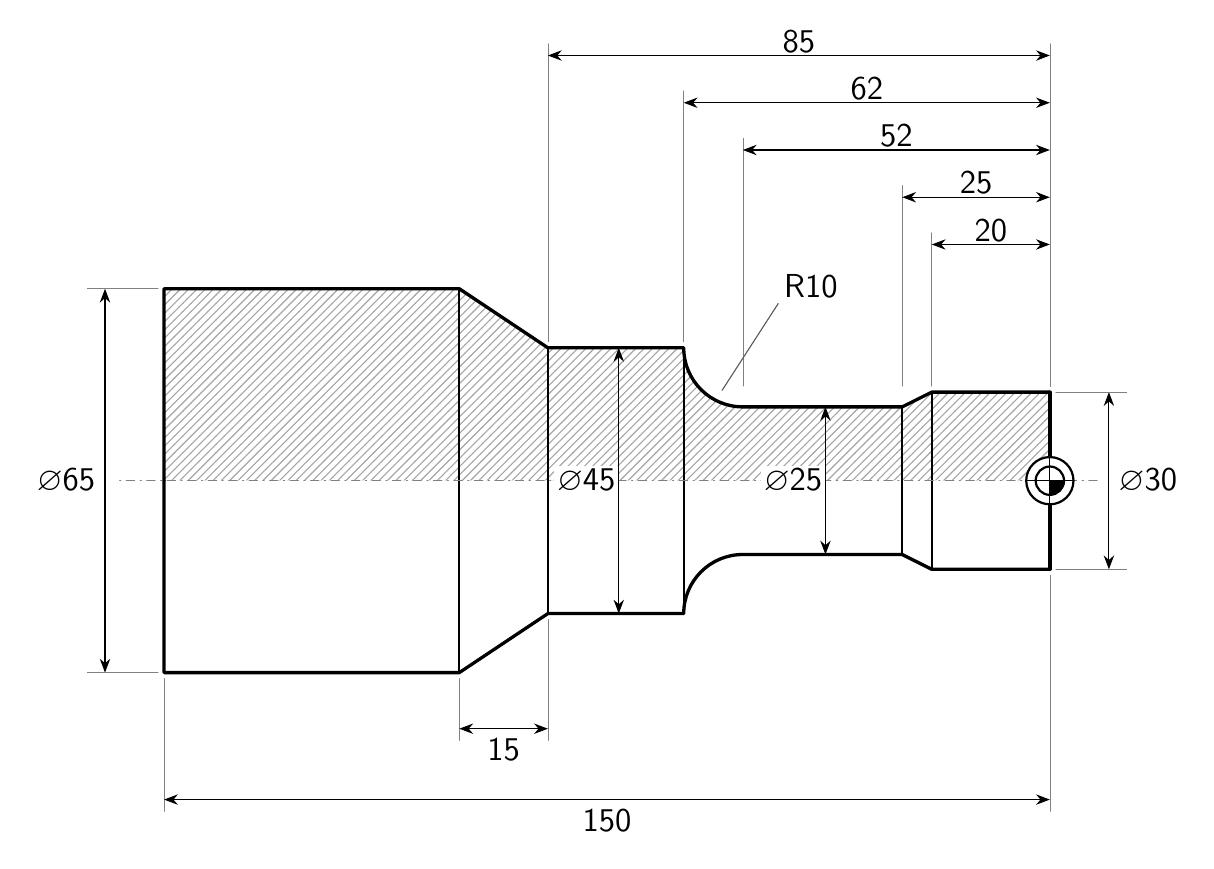
\begin{tikzpicture}[mm, x=0.075cm, y=0.075cm, font=\large]
  \fill[pattern=north east lines, pattern color=gray!70] \partprofile -- cycle;
  \fill[white] \partprofilelow -- cycle;
  \draw[very thick] \partprofile;
  \draw[very thick] \partprofilelow;
  \draw[very thick] (0,-15) -- (0,15);
  \foreach \z in {-20,-25,-52,-62,-85,-100} \draw[thin] (\z,-40) (\z,0) -- (\z,0);
  \draw[thick] (-20,-15) -- (-20,15) (-25,-12.5) -- (-25,12.5) (-62,-22.5) -- (-62,22.5)
               (-85,-22.5) -- (-85,22.5) (-100,-32.5) -- (-100,32.5);
  \draw[dash dot, gray] (8,0) -- (-158,0);
  \pic at (0,0) {wporigin};
  % diameters (right side and left side)
  \draw[dim] (10,-15) -- node[right] {$\varnothing$30} (10,15);
  \draw[ext] (1,15) -- (13,15) (1,-15) -- (13,-15);
  \draw[dim] (-38,-12.5) -- node[left, fill=white, inner sep=1pt] {$\varnothing$25} (-38,12.5);
  \draw[dim] (-73,-22.5) -- node[left, fill=white, inner sep=1pt] {$\varnothing$45} (-73,22.5);
  \draw[dim] (-160,-32.5) -- node[left] {$\varnothing$65} (-160,32.5);
  \draw[ext] (-151,32.5) -- (-163,32.5) (-151,-32.5) -- (-163,-32.5);
  % lengths from the right face (above the part)
  \foreach \z/\l/\h in {-20/20/40, -25/25/48, -52/52/56, -62/62/64, -85/85/72}{
    \draw[ext] (\z,{\z>-62 ? 16 : 23.5}) -- (\z,\h+2);
    \draw[ext] (0,16) -- (0,\h+2);
    \draw[dim] (0,\h) -- node[above, fill=white, inner sep=1pt] {\l} (\z,\h);}
  % below the part
  \draw[ext] (-100,-33.5) -- (-100,-44) (-85,-23.5) -- (-85,-44) (-150,-33.5) -- (-150,-56) (0,-16) -- (0,-56);
  \draw[dim] (-85,-42) -- node[below] {15} (-100,-42);
  \draw[dim] (0,-54) -- node[below] {150} (-150,-54);
  % fillet radius
  \draw[callout] (-55.5,15.3) -- (-46,30) node[above right=-2pt, black] {R10};
\end{tikzpicture}
\end{document}
